\documentclass{report}
\usepackage[utf8]{inputenc}    
\usepackage[T1]{fontenc}
\usepackage[francais]{babel}
\usepackage{wrapfig}
\usepackage{graphicx}
\usepackage{listings,xcolor}
\usepackage{appendix}
\usepackage{adjustbox}
\usepackage{titling}
\usepackage{float}
\usepackage{pdfpages}
\usepackage{caption}
\usepackage{subcaption}
\usepackage[hidelinks]{hyperref}
\usepackage{arydshln}
\usepackage{fixltx2e}
\usepackage{amsmath}

% Rotation de texte
\newcommand*\rot{\rotatebox{90}}
\newcommand*\halfrot{\rotatebox{135}}

% Alias pour texte en indice
\newcommand{\indice}{\textsubscript}

% Vecteur colonne
\newcommand{\colvect}[1]{\ensuremath{\begin{pmatrix}#1\end{pmatrix}}}


\hypersetup{
    colorlinks,
    citecolor=black,
    filecolor=black,
    linkcolor=blue,
    urlcolor=blue
}

%Géométrie des pages
\usepackage{geometry}
\geometry{hmargin=2.2cm,vmargin=2.2cm}

%Définition des couleurs pour le code xml
\definecolor{colorxmlnode}{rgb}{0.2, 0.2, 0.2} 
\definecolor{maroon}{RGB}{178 34 34}


%Profondeur des compteurs et de la tableofcontents
\setcounter{secnumdepth}{3}
\setcounter{tocdepth}{2}


%lst xml
\lstdefinelanguage{XML}
{
  basicstyle=\ttfamily,
  morestring=[s]{"}{"},
  morecomment=[s]{?}{?},
  morecomment=[s]{!--}{--},
  commentstyle=\color{darkgreen},
  moredelim=[s][\color{black}]{>}{<},
  moredelim=[s][\color{red}]{\ }{=},
  stringstyle=\color{blue},
  identifierstyle=\color{maroon}
}


\addto\captionsfrench{%
  \renewcommand\appendixname{Annexe}
  \renewcommand\appendixpagename{Annexes}
}

%Définition des commandes \noeud et \classe
\newcommand\classe[1]{\mbox{\textit{#1}}}
\newcommand\noeud[1]{\textcolor{colorxmlnode}{<\mbox{#1}>}}




\begin{document}

\begin{titlepage}
	\centering
	
    \vspace*{1.2 cm}
    
   	\textsc{\LARGE Master i informatique\\Travail Encadré de Recherche\\[0.3cm]\large Juin 2018}

	\vspace{2.2cm}
    
    
	\rule{\linewidth }{0.2 mm} \\[0.15 cm]
    {\LARGE \textbf{Rapport QuChemPedia}\\[0.2cm] \large
		\textbf{Sous titre}}\\
	\rule{\linewidth}{0.2 mm}
       \vspace*{0.1 cm}
	
	\begin{center}
	\vspace{0.3cm}
	
	\emph{Auteur}\\
	\vspace{0.1cm}
	Jules \bsc{Leguy}\\ 
	
	
	\vspace{0.5cm}
	\emph{Encadrants}\\
	\vspace{0.1cm}
	Benoit \bsc{Da Mota}\\
	Thomas \bsc{Cauchy}
	\end{center}		
	
	\vspace{1.0cm}


    
    
\end{titlepage}


\tableofcontents

\chapter{Introduction}
	\subsection{Motivation}

Les modèles décrits dans ce chapitre ont pour objectif de prédire la longueur de liaison optimisée entre des atomes partageant une liaison covalente au sein d'une molécule. L'objectif n'est donc pas de résoudre le problème de prédiction d'une géométrie moléculaire convergée complète, mais plutôt d'en résoudre une version locale simplifiée. Chronologiquement, cette classe de modèles est apparue après l'abandon des modèles tentant de prédire la géométrie optimisée complète d'une molécule (REF ABANDON DELTA\_DIST).\\
Puisque l'on résout le problème d'optimisation géométrique entre des couples d'atomes, la question de la façon d'utiliser cette méthode pour optimiser la géométrie complète d'une molécule se pose, nous n'y apportons cependant pas de réponse dans ce chapitre. L'objectif de ces modèles est en effet avant tout de valider notre capacité à effectuer des prédictions d'ordre géométrique de précision suffisante sur certains types de liaisons (REF GENERALISATION). L'élaboration d'une méthode d'optimisation géométrique moléculaire complète basée sur la résolution de sous-problèmes locaux est un problème très complexe, qui fait partie des nouveaux objectifs du projet QuChemPedia (REF PERSPECTIVES MODULES).\\
\par De plus, nous utilisons en entrée des modèles décrits dans ce chapitre des données « parfaites », c'est à dire qu'elles représentent des géométries déjà convergées. Ces données d'entrée ne correspondent donc pas aux données qui seraient utilisées dans un cas d'utilisation réel. L'utilisation de ces données permet cependant d'évaluer la capacité de nos modèles à effectuer des prédictions géométriques lorsque les conditions sont favorables, ce qui représente une première étape dans l'élaboration d'un système permettant de prédire les géométries convergées complètes (REF PERSPECTIVES MODULES).

\subsection{Représentation des données}

\subsubsection{Données en entrée des modèles}
\par Les modèles décrits dans ce chapitre utilisent en entrée la représentation géométrique locale des liaisons covalentes (REF GEOM LOCALE), qui permet de représenter les atomes au voisinage d'une liaison. En plus des informations géométriques, on représente la masse et le numéro atomique de chaque atome au voisinage de la liaison. Le numéro atomique est encodé en \emph{one-hot encoding}, c'est à dire de façon booléenne. La discrétisation des numéros atomiques a pour but de ne pas instaurer de relation d'ordre entre les différents atomes et donc a priori de mieux guider les modèles lors de l'apprentissage. Elle implique toutefois qu'il faut déterminer une limite aux numéros atomiques des atomes acceptés par un modèle. En effet, cet encodage coûte un attribut pour chaque numéro atomique accepté, pour chaque atome au voisinage de la liaison. Afin de travailler sur des modèles de taille raisonnable, ils acceptent les atomes de numéros atomiques inférieurs ou égaux à celui du fluor, ce qui correspond à neuf attributs encodant le numéro atomique pour chaque atome du voisinage.
\par De même la classe positionnelle (REF CLASSE POS) de chaque atome par rapport à la liaison est représenté en \emph{one-hot encoding}, afin de ne pas représenter cette information sur un ensemble possédant une relation d'ordre.\\

\par Le tableau suivant présente le nombre d'attributs utilisés pour représenter chaque atome au voisinage d'une liaison.

\begin{figure}[!h]
	\centering
	
	\begin{tabular}{|c|c|c|c|c|}
		\hline
		\textbf{Classe positionnelle} & \textbf{Distances} & \textbf{Masse atomique} & \textbf{Numéro atomique} & \textbf{Total}\\ \hline
		3 & 2 & 1 & 9 & 15\\ \hline
	\end{tabular}
	\caption{Quantité d'attributs représentant chaque atome au voisinage d'une liaison}
\end{figure}

\subsubsection{Homogénéisation de la taille des entrées}
\par Les molécules possédant un nombre variable d'atomes et l'entrée des modèles étant de taille fixe, nous effectuons une procédure de \emph{padding}\footnote{Rembourrage} des données. Cela signifie que l'entrée des modèles est découpée en blocs, représentant chacun un atome au voisinage de la liaison. La taille des blocs dépend des attributs représentant chaque atome, et le nombre de blocs définit le nombre maximal d'atomes au voisinage des liaisons que les modèles peuvent traiter. Nous déduisons cette information de la taille des molécules que l'on choisit d'accepter en entrée des modèles. La grande majorité des molécules étant de taille inférieure à 60 (VOIR DONNEES DISTRIB TAILLES) et les deux atomes composant la liaison n'apparaissant pas dans les entrées, nous choisissons de limiter le voisinage de la liaison à 58 atomes.\\
\par La représentation d'une liaison en entrée des modèles est donc composée de 58 blocs de 15 attributs, soit 870 valeurs. Lorsqu'une liaison possède moins de 58 voisins, les blocs correspondant aux atomes non définis valent zéro.

\subsubsection{Représentation d'une liaison en entrée d'un modèle}

\par Nous détaillons la représentation en entrée d'un modèle prédictif de la liaison imaginaire utilisée comme exemple en (REF REPR LOCALE). On considère que l'atome a$_3$ est un atome d'azote et que l'atome a$_4$ est un atome d'oxygène.

\vspace{0.5cm}

\begin{figure}[!h]
	\centering
	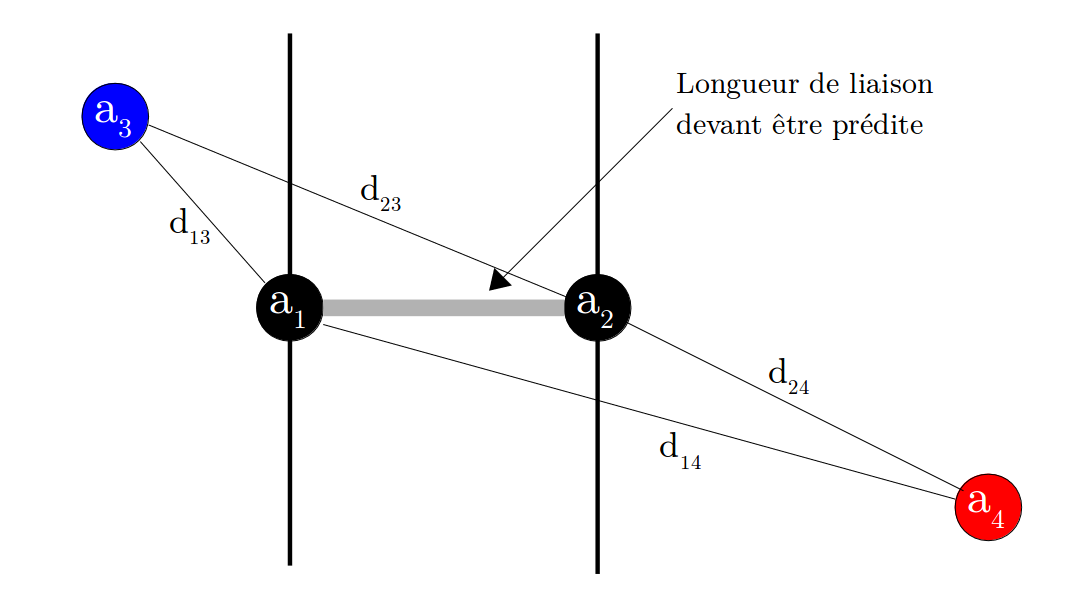
\includegraphics[scale=0.3]{images/classes_pos_4.png}
	\caption{Représentation schématique d'une liaison imaginaire}
\end{figure}

\par L'entrée correspondant à la liaison représentée ci-dessus est donnée dans le tableau suivant.

\begin{figure}[!h]
	\centering


	\begin{tabular}{|c|c|c|c|c|c|c|c|c|c|c|c|c|c|c|}
		\hline
		\multicolumn{3}{|c|}{\textbf{Classe pos.}} & \multicolumn{2}{|c|}{\textbf{Distances}} & \textbf{Masse atomique} & \multicolumn{9}{|c|}{\textbf{Numéro atomique}} \\
		\textbf{g?} & \textbf{c?} & \textbf{d?} & \multicolumn{2}{|c|}{}& & \textbf{H?} & \textbf{He?} & \textbf{Li?} & \textbf{Be?} & \textbf{B? }& \textbf{C?} & \textbf{N?} & \textbf{O?} & \textbf{F?} \\ \hline
		1 & 0 & 0 & $d_{13}$ & $d_{23}$ & 14,007 & 0 & 0 & 0 & 0 & 0 & 0 & 1 & 0 & 0 \\ \hline
		0 & 0 & 1 & $d_{14}$ & $d_{24}$ & 15,999 & 0 & 0 & 0 & 0 & 0 & 0 & 0 & 1 & 0 \\ \hline
		0 & 0 & 0 & 0 & 0 & 0 & 0 & 0 & 0 & 0 & 0 & 0 & 0 & 0 & 0 \\ \hline
		\rot{... } & \rot{... } & \rot{... } & \rot{... } & \rot{... } & \rot{... } & \rot{... } & \rot{... } & \rot{... } & \rot{... } & \rot{... } & \rot{... } & \rot{... } & \rot{... } & \rot{... }  \\ \hline 
		0 & 0 & 0 & 0 & 0 & 0 & 0 & 0 & 0 & 0 & 0 & 0 & 0 & 0 & 0 \\ \hline
	\end{tabular}

	\caption{Représentation des données d'une liaison en entrée d'un modèle prédictif}
\end{figure}



\subsection{Méthodologie}

\subsubsection{Précision requise}
\par Les modèles décrits dans ce chapitre travaillent sur des données « parfaites », c'est à dire qu'il prédisent des longueurs de liaisons dans des molécules dont la géométrie a déjà été optimisée. Cela nous permet de confirmer notre capacité à effectuer des prédictions d'ordre géométrique, mais pas de nous assurer que les modèles pourront effectuer de bonnes prédictions sur des données non optimisées issues de mesures ou de résultats théoriques. L'entraînement de modèles travaillant sur des données imparfaites fera l'objet de la suite du projet QuChemPedia (REF PERSPECTIVES). Pour pouvoir espérer obtenir de bonnes prédictions sur des données non optimisées, il faut obtenir de très bons résultats sur des données optimisées, comme on le montre en REF GENERALISATION.

\par La précision que l'on peut espérer atteindre avec les données sur lesquelles les modèles s'entraînent (REF PUBCHEM) est de l'ordre du picomètre (pm), soit $10^{-12}$ m. Cette précision dépend des fonctions choisies lors de l'optimisation géométrique quantique des molécules (REF OPTI DFT). Les modèles effectuant des prédictions dont l'erreur est inférieure à 1 pm confirmeront donc notre capacité à effectuer des prédictions d'ordre géométrique de précision suffisante.

\subsubsection{Classes de modèles}
\par Nous tentons de prédire les longueurs de liaisons entre plusieurs couples d'atomes, en entraînant un modèle par couple d'atomes formant une liaison. Les liaisons carbone-carbone ne seront alors pas prédites par le même modèle que les liaisons carbone-hydrogène. Cette séparation en sous-problèmes segmentés a pour objectif d'évaluer la précision que peuvent atteindre les modèles sur les problèmes les plus simples que l'on peut leur donner. L'évaluation de leur précision sur des problèmes plus complexes fait partie des futurs objectifs (REF	MODULES PLUSIEURS LIAISONS). La prédiction des longueurs de liaisons d'un unique couple donné d'atomes par modèle n'en fait toutefois pas un problème trivial, car elles peuvent sensiblement varier en fonction des atomes impliqués (REF DISTRIB LONGUEURS). Si les liaisons oxygène-hydrogène ont une taille variant en général entre 97 pm et 102 pm soit avec une amplitude de 5 pm, la taille des liaisons carbone-carbone varie entre 120 pm et 160 pm, ce qui représente une amplitude de 40 pm. \\
\par L'entraînement des modèles est un processus qui prend un temps non négligeable (REF CONTRAINTES MATERIELLES). Pour cette raison, nous n'entraînons pas tous les modèles sur un grand nombre d'exemples et nous définissons deux classes de modèles ayant des objectifs différents. \\
\par La première classe de modèles a un objectif d'expérimentation. Les modèles sont entraînés sur un nombre relativement faible d'exemples différents sur 150 époques (REF DEF EPOCH), ce qui représente environ 2h de préparation de données et 6h d'entraînement avec le matériel disponible. Ces modèles sont entraînés dans le but d'expérimenter de nouveaux traitements des données d'entrée ou de nouveaux paramètres. Ils ont pour objectif de discriminer la qualité de ces entrées et paramètres, c'est pourquoi ils travaillent sur la prédiction difficile des distances de liaisons carbone-carbone. Ces modèles sont décrits en REF PRED C.	\\
\par La seconde classe de modèles a un objectif de validation des paramètres performants issus de l'entraînement des modèles de la première classe, ainsi qu'un objectif de généralisation des méthodes à différents types de liaisons. Ces modèles s'entraînent donc sur plus d'exemples et sur plusieurs liaisons différentes (carbone-carbone, carbone-hydrogène et oxygène-hydrogène). L'entraînement des trois modèles de cette classe pour un ensemble d'entrées et de paramètres donné prend environ deux jours. Ces modèles sont décrits en REF GENERALISATION.

\subsection{Nomenclature}
\par Afin d'y faire référence simplement, nous nommons les différents modèles que l'on entraîne. Tous les modèles décrits dans ce chapitre ont pour préfixe \emph{DIST\_REL}, issu de leur vocation à prédire la distance relative entre les atomes d'une liaison, et pour suffixe le numéro chronologique de leur entraînement au sein de leur classe.\\
Les modèles de la première classe (resp. seconde) ont pour préfixe \emph{DIST\_REL\_C} (resp. \emph{DIST\_REL\_XY}, où X et Y désignent les symboles des éléments formant la liaison prédite). La différence de nomenclature entre les deux classes et notamment entre les modèles \emph{DIST\_REL\_C} et \emph{DIST\_REL\_CC} est discutable, mais a pour avantage de faire apparaître simplement la distinction.\\
Enfin, les modèles prédictifs n'étant pas des réseaux de neurones artificiels font apparaître leur type dans leur nom.


\chapter{Description des problèmes}
		
\chapter{Représentations géométriques moléculaires}
	\section{Matrice des coordonnées}
		\par La matrice des coordonnées atomiques est la façon la plus simple de représenter la géométrie d'une molécule. L'intérêt de cette représentation est qu'elle est utilisée par les chimistes (fichiers .mol, .xyz + utilisation dans les logiciels de calcul ?). Il s'agit donc pour nous d'une représentation d'entrée et de sortie. Nos données d'apprentissage contiennent pour chaque molécule une matrice des positions, en plus des numéros et masses atomiques, et nous devons être capables de fournir cette représentation en sortie de nos prédictions, pour que nos résultats soient utilisables par les chimistes.\\

\par Formellement, la matrice des coordonnées atomiques d'une molécule contient les coordonnées de chaque atome dans un repère cartésien orthonormé à trois dimensions.

\begin{figure}[!h]
	\centering
	
	\begin{tabular}{|c|c|c|}
		\hline
		$\boldsymbol{x_1}$ & $\boldsymbol{y_1}$ & $\boldsymbol{z_1}$ \\ \hline	
		$\boldsymbol{x_2}$ & $\boldsymbol{y_2}$ & $\boldsymbol{z_2}$ \\ \hline	
		\textbf{\rot{... }} & \textbf{\rot{... }} & \textbf{\rot{... }}\\ \hline 	
		$\boldsymbol{x_n}$ & $\boldsymbol{y_n}$ & $\boldsymbol{z_n}$ \\ \hline	
	\end{tabular}

	\caption{Matrice des coordonnées atomiques (molécule de taille $n$)}
\end{figure}

\par Si cette représentation de la géométrie des molécules est très commode pour les chimistes, elle n'est pas utilisable telle quelle dans nos modèles prédictifs. Nous cherchons en effet à prédire des distances (ou des différences de distances, voir REF DELTA\_DIST...) entre des points. Donner les coordonnées  brutes aux modèles implique qu'ils devraient \emph{apprendre} les outils mathématiques permettant de calculer des distances entre des points, ce qui constitue en soi une tâche complexe. C'est pourquoi nous allons définir un ensemble de représentations géométriques, toutes basées sur les distances plutôt que les positions, et adaptées aux différentes prédictions que nous souhaitons effectuer.

	\section{Matrice réduite des distances inter-atomiques}
		\subsection{Motivation}

\par Cette représentation est issue du travail qui a été fait précédemment sur ce projet, et consiste à représenter une molécule par ses distances inter-atomiques. L'intérêt de cette représentation est que les réseaux de neurones qui l'utilisent travaillent dans des repères relatifs. Lorsqu'ils effectuent des prédictions, ils n'ont pas besoin de \textit{comprendre} les notions mathématiques de géométrie permettant de déduire la position d'un point dans un repère à partir de ses distances à d'autres points, contrairement à la représentation décrite en (REF REPR ABS). Cette représentation est donc très commode pour les modèles prédictifs dont l'objectif est de corriger les distances entre deux atomes, puisqu'elle est basée sur les distances entre les paires d'atomes.

\par De plus, l'utilisation d'une représentation basée sur les distances relatives permet d'offrir une représentation unique pour les molécules ayant des ensembles d'atomes pouvant effectuer des rotations, contrairement aux représentations basées sur les coordonnées (REF REPR COORDS) ou sur des distances à des points fixes (REF REPR DIST ABS).

\par Lorsque les modèles utilisent cette représentation en sortie, ou plus précisément que l'on déduit la matrice réduite des distances inter-atomiques de la sortie du modèle (voir REF SORTIE DELTA\_DIST+H), nous devons toutefois trouver une méthode (voir REF PRINC RECONSTRUCT) pour reconstruire les molécules sous la forme d'une matrice de coordonnées (REF REPR COORDS).

\subsection{Formalisation}

\par Pour ne pas surcharger les modèles d'information, nous ne travaillons pas sur la matrice de distances inter-atomiques complète, mais sur un sous-ensemble de cardinalité minimale de cette matrice telle que nous pouvons reconstruire sans ambiguïté un ensemble de coordonnées représentant les positions des atomes de la molécule. La matrice des distances étant symétrique et la diagonale étant nulle, toute l'information est contenue dans chaque demi-matrice triangulaire privée de la diagonale. \\

\begin{figure}[h!]
	\centering
	
	
	\begin{tabular}{c|c|c|c|c|c|c|c|c|c|c|c|c}
	    & a\textsubscript{0} & a\textsubscript{1} & a\textsubscript{2} & a\textsubscript{3} & a\textsubscript{4} & ... & a\textsubscript{n-4} & a\textsubscript{n-3} & a\textsubscript{n-2} & 
	    	 a\textsubscript{n-1}  & a\textsubscript{n}\\ \hline
		a\textsubscript{0} & \textbf{d\textsubscript{0,0}} & \textbf{d\textsubscript{0,1}} & \textbf{d\textsubscript{0,2}} & 
		    \textbf{d\textsubscript{0,3}} & \textbf{d\textsubscript{0,4}} & \textbf{...} & \textbf{d\textsubscript{0,n-4}} & 
		    \textbf{d\textsubscript{0,n-3}} & \textbf{d\textsubscript{0,n-2}} & \textbf{d\textsubscript{0,n-1}}
		    & \textbf{d\textsubscript{0,n}} \\ \hline
		a\textsubscript{1} & \textbf{d\textsubscript{1,0}} & \textbf{d\textsubscript{1,1}} & \textbf{d\textsubscript{1,2}} & 
			\textbf{d\textsubscript{1,3}} & \textbf{d\textsubscript{1,4}} & \textbf{...} & \textbf{d\textsubscript{1,n-4}} & 
			\textbf{d\textsubscript{1,n-3}} & \textbf{d\textsubscript{1,n-2}} & \textbf{d\textsubscript{1,n-1}} & 
			\textbf{d\textsubscript{1,n}} \\ \hline
		a\textsubscript{2} & \textbf{d\textsubscript{2,0}} & \textbf{d\textsubscript{2,1}} & \textbf{d\textsubscript{2,2}} &
			\textbf{d\textsubscript{2,3}} & \textbf{d\textsubscript{2,4}} & \textbf{...} & \textbf{d\textsubscript{2,n-4}} & 
			\textbf{d\textsubscript{2,n-3}} & \textbf{d\textsubscript{2,n-2}} & \textbf{d\textsubscript{2,n-1}} & 
			\textbf{d\textsubscript{2,n}} \\ \hline
		a\textsubscript{3} & \textbf{d\textsubscript{3,0}} & \textbf{d\textsubscript{3,1}} & \textbf{d\textsubscript{3,2}} & 
			\textbf{d\textsubscript{3,3}} & \textbf{d\textsubscript{3,4}} & \textbf{...} & \textbf{d\textsubscript{3,n-4}} & 
			\textbf{d\textsubscript{3,n-3}} & \textbf{d\textsubscript{3,n-2}} & \textbf{d\textsubscript{3,n-1}} & 
			\textbf{d\textsubscript{3,n}} \\ \hline
		a\textsubscript{4} & \textbf{d\textsubscript{4,0}} & \textbf{d\textsubscript{4,1}} & \textbf{d\textsubscript{4,2}} & 
			\textbf{d\textsubscript{4,3}} & \textbf{d\textsubscript{4,4}} & \textbf{...} & \textbf{d\textsubscript{4,n-4}} & 
			\textbf{d\textsubscript{4,n-3}} & \textbf{d\textsubscript{4,n-2}} & \textbf{d\textsubscript{4,n-1}} & 
			\textbf{d\textsubscript{4,n}} \\ \hline
			
		\rot{... } & \textbf{\rot{... }} & \textbf{\rot{... }} & \textbf{\rot{... }} & \textbf{\rot{... }} & 
		\textbf{\rot{... }} & \textbf{\halfrot{ ... }} & \textbf{\rot{... }} & \textbf{\rot{... }} & \textbf{\rot{... }} & 
		\textbf{\rot{... }} & \textbf{\rot{... }} \\ \hline


		a\textsubscript{n-4} & \textbf{d\textsubscript{n-4,0}} & \textbf{d\textsubscript{n-4,1}} & \textbf{d\textsubscript{n-4,2}} & 
			\textbf{d\textsubscript{n-4,3}} & \textbf{d\textsubscript{n-4,4}} & \textbf{...} & \textbf{d\textsubscript{n-4,n-4}} & 
			\textbf{d\textsubscript{n-4,n-3}} & \textbf{d\textsubscript{n-4,n-2}} & \textbf{d\textsubscript{n-4,n-1}} & 
			\textbf{d\textsubscript{n-3,n}} \\ \hline

		a\textsubscript{n-3} & \textbf{d\textsubscript{n-3,0}} & \textbf{d\textsubscript{n-3,1}} & \textbf{d\textsubscript{n-3,2}} & 
			\textbf{d\textsubscript{n-3,3}} & \textbf{d\textsubscript{n-3,4}} & \textbf{...} & \textbf{d\textsubscript{n-3,n-4}} & 
			\textbf{d\textsubscript{n-3,n-3}} & \textbf{d\textsubscript{n-3,n-2}} & \textbf{d\textsubscript{n-3,n-1}} & 
			\textbf{d\textsubscript{n-3,n}} \\ \hline
		a\textsubscript{n-2} & \textbf{d\textsubscript{n-2,0}} & \textbf{d\textsubscript{n-2,1}} & \textbf{d\textsubscript{n-2,2}} & 
			\textbf{d\textsubscript{n-2,3}} & \textbf{d\textsubscript{n-2,4}} & \textbf{...} & \textbf{d\textsubscript{n-2,n-4}} & 
			\textbf{d\textsubscript{n-2,n-3}} & \textbf{d\textsubscript{n-2,n-2}} & \textbf{d\textsubscript{n-2,n-1}} & 
			\textbf{d\textsubscript{n-2,n}} \\ \hline
		a\textsubscript{n-1} & \textbf{d\textsubscript{n-1,0}} & \textbf{d\textsubscript{n-1,1}} & \textbf{d\textsubscript{n-1,2}} & 
			\textbf{d\textsubscript{n-1,3}} & \textbf{d\textsubscript{n-1,4}} & \textbf{...} & \textbf{d\textsubscript{n-1,n-4}} & 
			\textbf{d\textsubscript{n-1,n-3}} & \textbf{d\textsubscript{n-1,n-2}} & \textbf{d\textsubscript{n-1,n-1}} & 
			\textbf{d\textsubscript{n-1,n}} \\ \hline
		a\textsubscript{n} & \textbf{d\textsubscript{n,0}} & \textbf{d\textsubscript{n,1}} & \textbf{d\textsubscript{n,2}} & 
			\textbf{d\textsubscript{n,3}} & \textbf{d\textsubscript{n,4}} & \textbf{...} & \textbf{d\textsubscript{n,n-4}} & 
			\textbf{d\textsubscript{n,n-3}} & \textbf{d\textsubscript{n,n-2}} & \textbf{d\textsubscript{n,n-1}} & 
			\textbf{d\textsubscript{n,n}} \\ \hline
		
	\end{tabular}

	
	\caption{Matrice complète des distances inter-atomiques d'une molécule}
\end{figure}

\par De plus, nous n'avons besoin que des distances à quatre points pour retrouver la position de chaque atome (voir REF RECONSTRUCT), nous nous contentons donc de garder les quatre premières distances de chaque ligne de la matrice triangulaire supérieure privée de la diagonale.


\begin{figure}[h!]
	\centering
	
	
	\begin{tabular}{c|c|c|c|c|c|c|c|c|c|c|c|c}
	    & a\textsubscript{0} & a\textsubscript{1} & a\textsubscript{2} & a\textsubscript{3} & a\textsubscript{4} & ... & a\textsubscript{n-4} & a\textsubscript{n-3} & a\textsubscript{n-2} & 
	    	 a\textsubscript{n-1}  & a\textsubscript{n}\\ \hline
		a\textsubscript{0} & d\textsubscript{0,0} & \textbf{d\textsubscript{0,1}} & \textbf{d\textsubscript{0,2}} & 
		    \textbf{d\textsubscript{0,3}} & \textbf{d\textsubscript{0,4}} & ... & d\textsubscript{0,n-4} & 
		    d\textsubscript{0,n-3} & d\textsubscript{0,n-2} & d\textsubscript{0,n-1}
		    & d\textsubscript{0,n} \\ \hline
		a\textsubscript{1} & d\textsubscript{1,0} & d\textsubscript{1,1} & \textbf{d\textsubscript{1,2}} & 
			\textbf{d\textsubscript{1,3}} & \textbf{d\textsubscript{1,4}} & ... & d\textsubscript{1,n-4} & 
			d\textsubscript{1,n-3} & d\textsubscript{1,n-2} & d\textsubscript{1,n-1} & 
			d\textsubscript{1,n} \\ \hline
		a\textsubscript{2} & d\textsubscript{2,0} & d\textsubscript{2,1} & d\textsubscript{2,2} &
			\textbf{d\textsubscript{2,3}} & \textbf{d\textsubscript{2,4}} & ... & d\textsubscript{2,n-4} & 
			d\textsubscript{2,n-3} & d\textsubscript{2,n-2} & d\textsubscript{2,n-1} & 
			d\textsubscript{2,n} \\ \hline
		a\textsubscript{3} & d\textsubscript{3,0} & d\textsubscript{3,1} & d\textsubscript{3,2} & 
			d\textsubscript{3,3} & \textbf{d\textsubscript{3,4}} & ... & d\textsubscript{3,n-4} & 
			d\textsubscript{3,n-3} & d\textsubscript{3,n-2} & d\textsubscript{3,n-1} & 
			d\textsubscript{3,n} \\ \hline
			
		a\textsubscript{4} & d\textsubscript{4,0} & d\textsubscript{4,1} & d\textsubscript{4,2} & 
			d\textsubscript{4,3} & \textbf{d\textsubscript{4,4}} & ... & d\textsubscript{4,n-4} & 
			d\textsubscript{4,n-3} & d\textsubscript{4,n-2} & d\textsubscript{4,n-1} & 
			d\textsubscript{4,n} \\ \hline
			
		\rot{... } & \rot{... } & \rot{... } & \rot{... } & \rot{... } & 
		\rot{... } & \halfrot{ ... } & \rot{... } & \rot{... } & \rot{... } & 
		\rot{... } & \rot{... } \\ \hline
	    	
	    	
		a\textsubscript{n-4} & d\textsubscript{n-4,0} & d\textsubscript{n-4,1} & d\textsubscript{n-4,2} & 
			d\textsubscript{n-4,3} & d\textsubscript{n-4,4} & ... & d\textsubscript{n-4,n-4} & 
			\textbf{d\textsubscript{n-4,n-3}} & \textbf{d\textsubscript{n-4,n-2}} & \textbf{d\textsubscript{n-4,n-1}} & 
			\textbf{d\textsubscript{n-4,n}} \\ \hline	    
		a\textsubscript{n-3} & d\textsubscript{n-3,0} & d\textsubscript{n-3,1} & d\textsubscript{n-3,2} & 
			d\textsubscript{n-3,3} & d\textsubscript{n-3,4} & ... & d\textsubscript{n-3,n-4} & 
			d\textsubscript{n-3,n-3} & \textbf{d\textsubscript{n-3,n-2}} & \textbf{d\textsubscript{n-3,n-1}} & 
			\textbf{d\textsubscript{n-3,n}} \\ \hline
		a\textsubscript{n-2} & d\textsubscript{n-2,0} & d\textsubscript{n-2,1} & d\textsubscript{n-2,2} & 
			d\textsubscript{n-2,3} & d\textsubscript{n-2,4} & ... & d\textsubscript{n-2,n-4} & 
			d\textsubscript{n-2,n-3} & d\textsubscript{n-2,n-2} & \textbf{d\textsubscript{n-2,n-1}} & 
			\textbf{d\textsubscript{n-2,n}} \\ \hline
		a\textsubscript{n-1} & d\textsubscript{n-1,0} & d\textsubscript{n-1,1} & d\textsubscript{n-1,2} & 
			d\textsubscript{n-1,3} & d\textsubscript{n-1,4} & ... & d\textsubscript{n-1,n-4} & 
			d\textsubscript{n-1,n-3} & d\textsubscript{n-1,n-2} & d\textsubscript{n-1,n-1} & 
			\textbf{d\textsubscript{n-1,n}} \\ \hline
		a\textsubscript{n} & d\textsubscript{n,0} & d\textsubscript{n,1} & d\textsubscript{n,2} & 
			d\textsubscript{n,3} & d\textsubscript{n,4} & ... & d\textsubscript{n,n-4} & 
			d\textsubscript{n,n-3} & d\textsubscript{n,n-2} & d\textsubscript{n,n-1} & d\textsubscript{n,n} \\ \hline
		
	\end{tabular}

	
	\caption{Matrice réduite des distances inter-atomiques d'une molécule (en gras)}
\end{figure}

\begin{figure}[h!]
	\centering
	
	
	\begin{tabular}{|c|c|c|c|}
		\hline
		\textbf{d\textsubscript{0,1}} & \textbf{d\textsubscript{0,2}} & \textbf{d\textsubscript{0,3}} & \textbf{d\textsubscript{0,4}} \\ \hline
		\textbf{d\textsubscript{1,2}} & \textbf{d\textsubscript{1,3}} & \textbf{d\textsubscript{1,4}} & \textbf{d\textsubscript{1,5}} \\ \hline
		\textbf{d\textsubscript{2,3}} & \textbf{d\textsubscript{2,4}} & \textbf{d\textsubscript{2,5}} & \textbf{d\textsubscript{2,6}} \\ \hline
		\textbf{d\textsubscript{3,4}} & \textbf{d\textsubscript{3,5}} & \textbf{d\textsubscript{3,6}} & \textbf{d\textsubscript{3,7}} \\ \hline
		\textbf{\rot{... }} & \textbf{\rot{... }} & \textbf{\rot{... }} & \textbf{\rot{... }} \\ \hline
		\textbf{d\textsubscript{n-4,n-3}} & \textbf{d\textsubscript{n-4,n-2}} & \textbf{d\textsubscript{n-4,n-1}} & \textbf{d\textsubscript{n-4,n}} \\ \hline
		\textbf{d\textsubscript{n-3,n-2}} & \textbf{d\textsubscript{n-3,n-1}} & \textbf{d\textsubscript{n-3,n}} & \textbf{0} \\ \hline
		\textbf{d\textsubscript{n-2,n-1}} & \textbf{d\textsubscript{n-2,n}} & \textbf{0} & \textbf{0} \\ \hline
		\textbf{d\textsubscript{n-1,n}} & \textbf{0} & \textbf{0} & \textbf{0} \\ \hline
	\end{tabular}

	
	\caption{Matrice réduite des distances inter-atomiques d'une molécule}
\end{figure}

\newpage
\subsection{Reconstruction des molécules}

\par Lorsqu'un modèle a pour sortie une matrice réduite des distances inter-atomiques lorsqu'il effectue des prédictions, il faut définir une méthode pour reconstruire une matrice des coordonnées (ref REPR MAT COORDS) de façon automatique à partir de cette sortie, la seule contrainte étant que la distance relative entre chaque paire d'atomes soit respectée. Il ne s'agit pour autant pas d'une tâche triviale, elle s'est en effet avérée impossible en pratique pour les grosses molécules à cause de la propagation des erreurs qu'elle induit (voir REF PROPAG ERREURS).

\subsubsection{Formalisation de la méthode de reconstruction}

\paragraph{Nécessité et limite de l'introduction d'un atome fictif} Notre méthode de reconstruction des atomes doit permettre de respecter la chiralité\footnote{Un composé chimique est dit chiral s'il n'est pas superposable à son image dans un miroir. (\url{https://fr.wikipedia.org/wiki/Chiralité_(chimie))}} des molécules. Or, en déduisant uniquement la position d'un atome de ses distances aux quatre atomes précédents, il existe des cas pour lesquels il existe plusieurs solutions pour la position de l'atome (deux si les quatre atomes précédents sur un même plan ou une infinité si les quatre atomes précédents appartiennent à une droite). Pour pallier ce problème, la méthode retenue précédemment a été d'introduire un nouveau point (que l'on nomme atome fictif) et que l'on place arbitrairement dans la molécule, à une position telle qu'il n'appartient pas au plan formé par les trois premiers atomes, ou à la droite formée par les trois premiers atomes s'ils sont alignés. De cette façon, les atomes suivants seront placés sans ambiguïté.\\
Cependant, on peut imaginer des cas pour lesquels la technique de l'introduction d'un atome fictif ne permet pas de lever l'ambiguïté, notamment pour les molécules possédant une chaîne de carbones liés par des doubles liaisons (et formant donc une droite). La méthode ne permettra pas dans ce cas de déterminer les positions des atomes en bout de chaîne tel que leurs distances relatives soient respectées, cette information étant perdue lors de la création de la matrice réduite des distances inter-atomiques. \\
Cette représentation n'est donc pas viable en pratique. Cela fait partie des raisons (voir également REF PB SQRT) pour lesquelles nous sommes passés à la représentation par matrice réduite des distances à des points fixes (REF MATR RED FIXES).

\paragraph{Placement de l'atome fictif} Puisque l'on définit la position de chaque atome en fonction de ses distances aux quatre atomes précédents, on doit d'abord placer les quatre premiers atomes de façon partiellement arbitraire. Le premier atome de la molécule dans notre représentation étant l'atome fictif a\indice{0}, nous commençons par le placer à la position qui lui a été attribuée.

\paragraph{Placement de l'atome a\indice{1}} Une fois l'atome a\indice{0} placé, il existe une infinité de solutions pour la position de l'atome a\indice{1}. On peut en effet le placer à tout point appartenant à la surface de la sphère de centre a\indice{0} et de rayon d\indice{0,1}.



\paragraph{Placement de l'atome a\indice{2}} L'atome a\indice{2} appartient au cercle solution de l'intersection entre les sphères de centres a\indice{0} et a\indice{1} et de rayons d\indice{0,2} et d\indice{1,2}. On choisit donc arbitrairement une position appartenant à ce cercle.



\paragraph{Placement de l'atome a\indice{3}} Dans le cas général, il existe deux solutions pour le placement de l'atome a\indice{3}, l'intersection non nulle de trois sphères étant deux points si tous les points ne sont pas sur un même plan ou une même droite. On choisit arbitrairement un point parmi ces deux solutions, car il n'y a pas à ce stade d'ambiguïté de chiralité de la molécule, une molécule composée de trois atomes ne possédant pas de chiralité (l'atome fictif a\indice{0} ne fait pas partie de la molécule).


\paragraph{Placement de l'atome a\indice{n}} Pour placer l'atome a\indice{$n$} ($n$ étant strictement inférieur à la taille de la molécule), nous généralisons la méthode de placement de l'atome a\indice{3}. Plutôt que de travailler sur l'intersection de quatre sphères, nous travaillons toujours sur l'intersection de trois sphères et nous utilisons la dernière distance pour discriminer les deux solutions obtenues. Cela facilite grandement la résolution des équations mathématiques associées et permet d'obtenir des solutions sensiblement équivalentes. \\
Formellement, nous calculons les positions des deux points solutions de l'intersection des trois sphères de centres a\indice{n-4}, a\indice{n-3}, et a\indice{n-2} et de rayons d\indice{n-4,n}, d\indice{n-3,n} et d\indice{n-2,n}, et nous discriminons les deux solutions selon la distance d\indice{n-1,n}. 

\begin{figure}
	\centering
	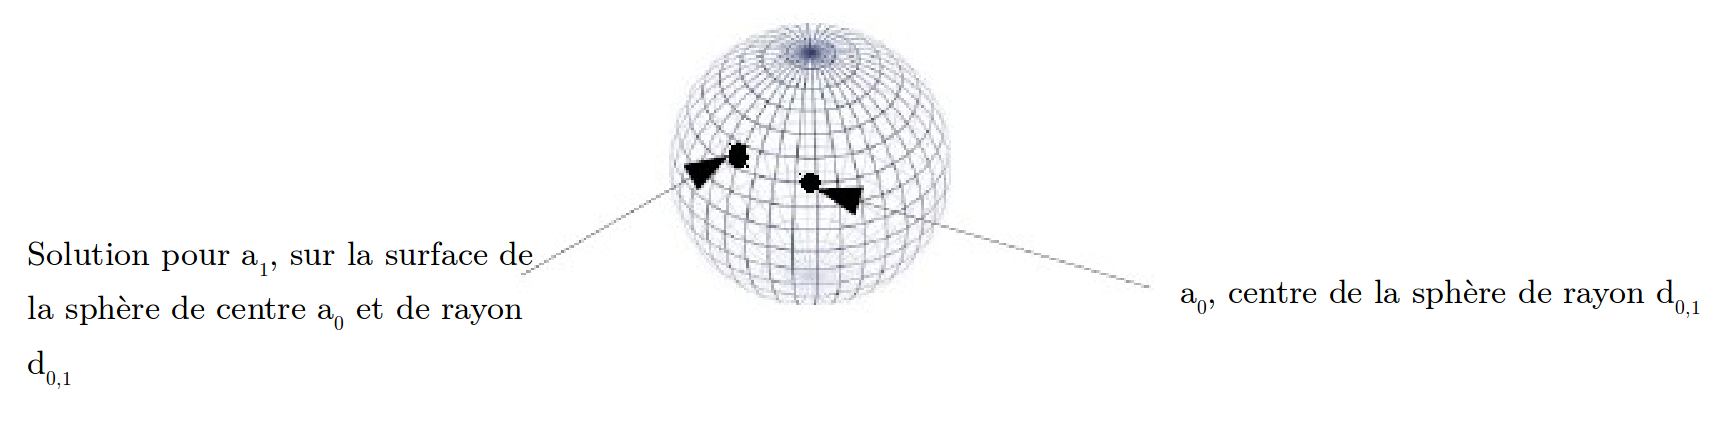
\includegraphics[scale=0.27]{images/1_sphere.png}
	\caption{Placement de l'atome a\indice{1} (image extraite du rapport de N.Roux)}
\end{figure}

\begin{figure}
	\centering
	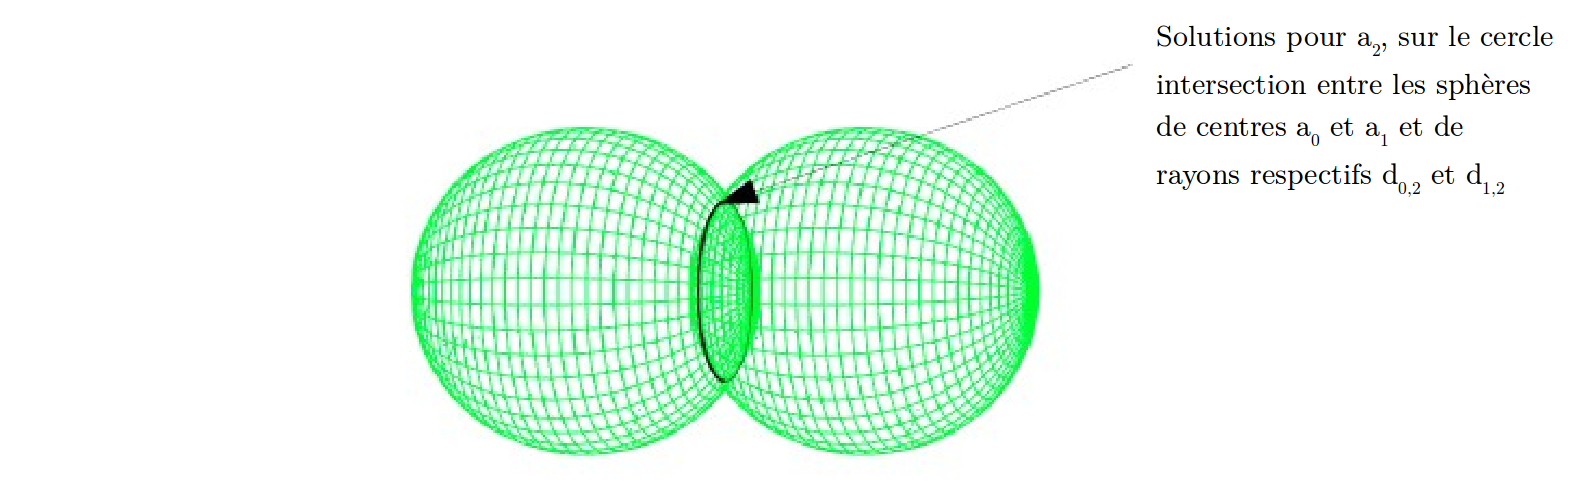
\includegraphics[scale=0.3]{images/2_spheres.png}
	\caption{Placement de l'atome a\indice{2} (image extraite du rapport de N.Roux)}
\end{figure}


\begin{figure}
	\centering
	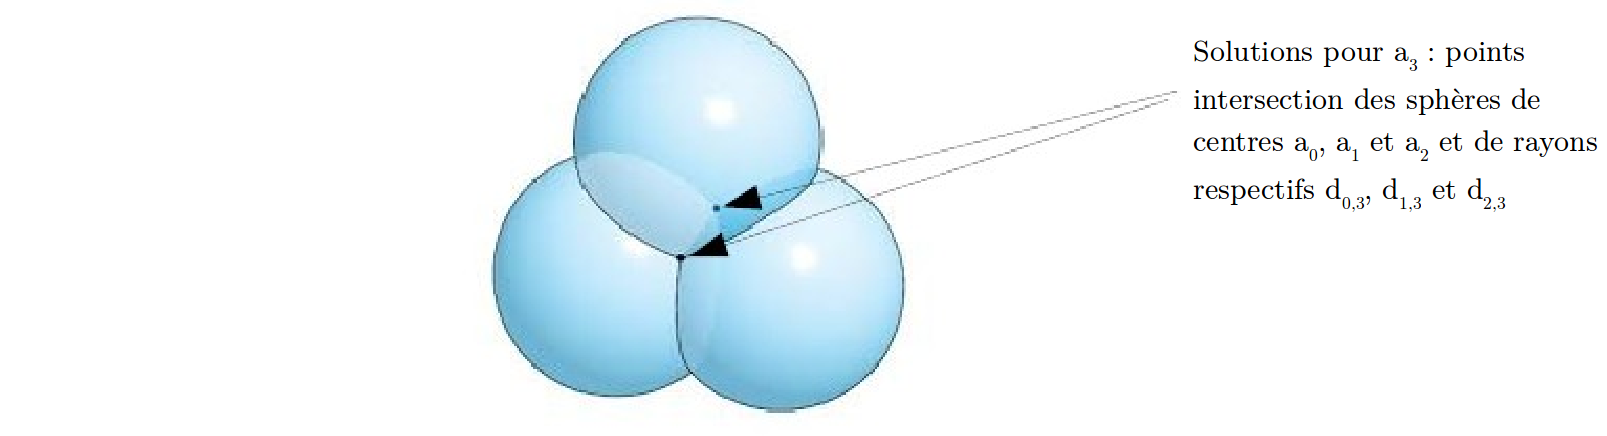
\includegraphics[scale=0.3]{images/3_spheres.png}
	\caption{Placement de l'atome a\indice{3} (image extraite du rapport de N.Roux)}
\end{figure}


\begin{figure}
	\centering
	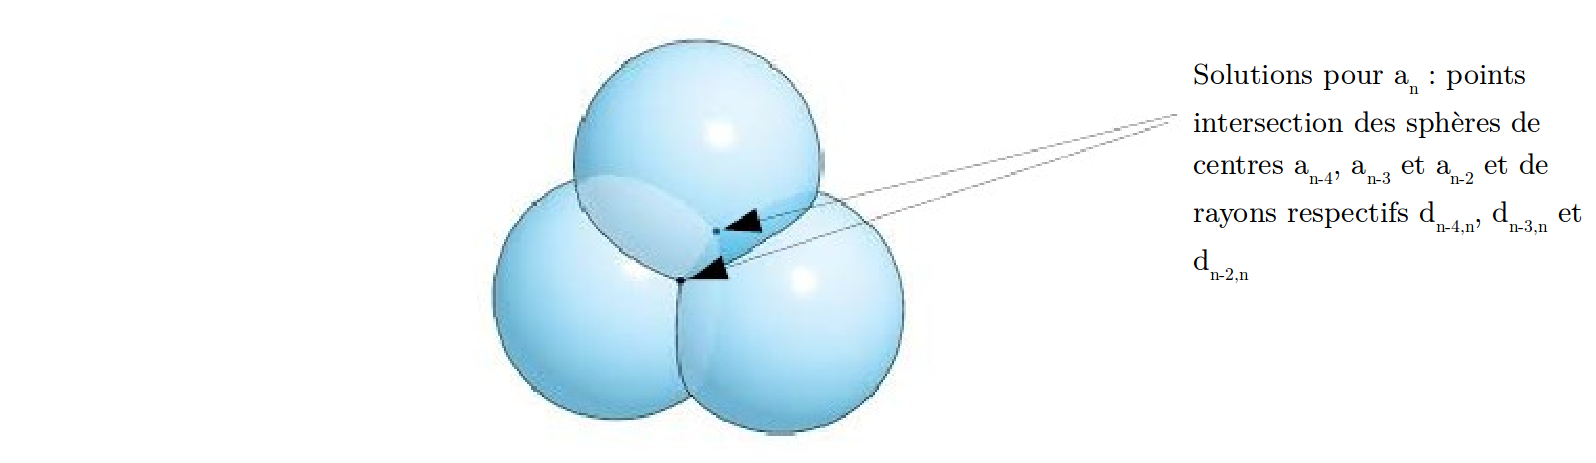
\includegraphics[scale=0.3]{images/3_spheres_gen.png}
	\caption{Placement de l'atome a\indice{n} (image extraite du rapport de N.Roux)}
\end{figure}

\subsubsection{Reconstruction automatique des positions en utilisant un solveur}

\par Nous développons ici une méthode permettant de déterminer les coordonnées d'un atome quelconque en utilisant un solveur d'équations non linéaires \footnote{\url{https://en.wikipedia.org/wiki/Nonlinear_system}}. Nous utilisons la bibliothèque Sympy\footnote{\url{http://www.sympy.org/fr/}}.\\

\par Tout d'abord, l'atome fictif a\indice{0} doit être placé à la position qui lui a été attribuée (REF PLACEMENT AT FICTIF). Nous plaçons ensuite arbitrairement les trois atomes suivants, de sorte que leurs distances relatives soient respectées. Pour simplifier le problème, nous effectuons une translation temporaire telle que a\indice{0}$'$ est à l'origine du repère. Nous plaçons alors a\indice{1}$'$ sur l'axe $x$, à une distance d\indice{0,1} de l'origine, et a\indice{2}$'$ sur le plan tel que $z=0$, à une position telle que les distances d\indice{0,2} et d\indice{1,2} sont respectées. Pour finir, nous plaçons a\indice{3}$'$ à l'une des deux solutions de l'intersection des sphères associées au problème (REF PLACEMENT A3). Le choix de la solution est arbitraire car la reconstruction de la bonne chiralité de la molécule ne dépend pas du placement des trois premiers atomes non fictifs.\\



\begin{figure}[!h]
	\centering
	
	\[
	a_{0}'\left \{
   	\begin{array}{l}
      x_{0}'=0\\
      y_{0}'=0\\
	  z_{0}'=0
   	\end{array}
   	\right .
   	\:
   	a_{1}'\left \{
   	\begin{array}{l}
      x_{1}'=d_{0,1}\\
      y_{1}'=0\\
	  z_{1}'=0
   	\end{array}
   	\right .
   	\:
	a_{2}'\left \{
   	\begin{array}{l}
      x_{2}'=\frac{d_{0,2}^2 - d_{1,2}^2 + x_{1}^2}{2x_{1}'}\\
      y_{2}'=\sqrt{d_{2,0}^2 - x_{2}'^2}\\
	  z_{2}'=0
   	\end{array}
   	\right .
   	\:
   	a_{3}'\left \{
   	\begin{array}{l}
      x_{3}'=\frac{d_{0,3}^2+x_1'^2-d_{1,3}^2}{2x_{1}'}\\
      y_{3}'=\frac{-2x_3'x_2'+d_{0,2}^2-d_{2,3}^2+d_{0,3}^2}{2y_2'}\\
	  z_{3}'=\sqrt{-x_3'^2-y_3'^2+d_{0,3}^2}
   	\end{array}
   	\right .
	\]
		
	\caption{Placement des atomes a\indice{0}$'$, a\indice{1}$'$, a\indice{2}$'$ et a\indice{3}$'$}
\end{figure}


\par Une fois que les quatre premiers atomes sont placés, nous leur appliquons une translation selon le vecteur $\vec{a_0}$, de sorte que l'atome fictif soit à sa position originale, et que les distances relatives des atomes a\indice{0}, a\indice{1}, a\indice{2} et a\indice{3} soient toujours consistantes. Nous faisons alors appel au solveur pour résoudre les équations associées au placement des autres atomes de de la molécule. Pour chaque atome, nous sélectionnons la solution respectant au mieux la distance d\indice{n-1,n} (REF PLACEMENT AN).


\begin{figure}[!h]
	\centering
	
	\[
	\left \{
   	\begin{array}{l}
      d_{n-4,n}^2=(x_n-x_{n-4})^2 + (y_n-y_{n-4})^2 + (z_n-z_{n-4})^2\\
	  d_{n-3,n}^2=(x_n-x_{n-3})^2 + (y_n-y_{n-3})^2 + (z_n-z_{n-3})^2\\
      d_{n-2,n}^2=(x_n-x_{n-2})^2 + (y_n-y_{n-2})^2 + (z_n-z_{n-2})^2\\
   	\end{array}
   	\right .
	\]
	
	\caption{Équations de sphères permettant d'obtenir la position d'un atome quelconque de la molécule}
\end{figure}

\paragraph{Limites de l'approche par solveur} L'utilisation d'un solveur calculant les solutions au cas par cas pose deux problèmes importants. Le premier concerne les performances de la solution. En effet, la résolution des systèmes d'équations consomme beaucoup de ressources et prend donc un temps non négligeable si on souhaite appliquer la méthode à un grand nombre de molécules.\\
Le second problème est lié à la propagation des erreurs lors de la reconstruction (REF RECONSTRUCT TRILAT). À cause du manque de précision de certaines valeurs, certaines intersections de sphères sont vides. Le solveur renvoie alors des solutions imaginaires que nous ne pouvons pas interpréter. Ce problème se manifeste avant tout sur les molécules de taille importante, mais il est impossible de déterminer une taille limite au delà de laquelle nous ne pouvons pas reconstruire les molécules. Cela implique qu'il existe des molécules que nous ne pouvons pas reconstruire, et que nous ne pouvons pas déterminer à l'avance si une molécule donnée peut être reconstruite.

\begin{figure}[!h]
	\centering
	
	\begin{tabular}{|l|r|r|}
		
	
	\end{tabular}
	
	\caption{Temps d'exécution de la résolution par solveur}
\end{figure}

\subsubsection{Reconstruction automatique des positions en utilisant des équations de trilatération}

\par Afin de pallier les problèmes liés à l'utilisation d'un solveur pour construire l'ensemble des positions des atomes d'une molécule à partir de la matrice réduite des distances inter-atomiques, nous utilisons une méthode permettant de calculer les positions de chaque point à partir d'un ensemble d'équations. Cette méthode est décrite sur Wikipédia\footnote{\url{https://en.wikipedia.org/wiki/Trilateration}}. Il s'agit d'une méthode de trilatération de points, c'est à dire que l'on cherche à déterminer la position d'un point en fonction de ses distances à trois points dont les positions sont connues, par opposition à la triangulation\footnote{\url{https://fr.wikipedia.org/wiki/Triangulation}} pour laquelle on détermine la position d'un point en fonction de ses angles à des points dont les positions sont connues.\\

\par De même que pour la méthode utilisant un solveur (REF SOLV), nous commençons par placer l'atome fictif a\indice{0} à la position qui lui a été attribuée, puis les atomes a\indice{1}, a\indice{2} et a\indice{3} de façon arbitraire telle que les distances relatives des atomes a\indice{$i$}, $i \in \{0, ..., 3\}$ soient respectées. Nous utilisons pour cela les équations décrites en (REF FIG PLACEMENT).\\

\par Une fois les quatre premiers atomes placés, nous cherchons à placer l'atome a\indice{$n$} de la molécule en fonction de ses distances aux quatre atomes précédents. Nous calculons les solutions en considérant que $a\indice{n-4}'$ est à l'origine du repère, que $a\indice{n-3}'$ est sur l'axe $x$, et que $a\indice{n-2}'$ est sur le plan tel que $z=0$, puis nous effectuons une translation des solutions dans le système de coordonnées original. Pour cela, nous définissons les quantités et vecteurs suivants. 
\par La notation $\hat{u}$ indique un vecteur $u$ de norme 1, et nous considérons que $\overline{a_i}$ représente le vecteur allant de l'origine au point $a_i$, dans le but de simplifier l'écriture des équations.\\

\vspace{0.4cm}

\centerline{Vecteur unitaire dans la direction de $a_{n-4}$ à $a_{n-3}$ :}

\[
\hat{e_x} = \frac{\overline{a_{n-3}}-\overline{a_{n-4}}}{d_{n-4,n-3}}
\]

\vspace{0.4cm}

\centerline{Ordre de grandeur signé de la composante $x$ dans le nouveau}
\centerline{ système de coordonnées du vecteur $\overline{a_{n-4}a_{n-2}}$ : }
\[
i = \hat{e_x}\cdot(\overline{a_{n-4}}-\overline{a_{n-2}})
\]

\vspace{0.4cm}

\centerline{Vecteur unitaire dans la direction $y$ par rapport à $\hat{e_x}$:}
\[
\hat{e_y} = \frac{\overline{a_{n-2}}-\overline{a_{n-4}}-i\hat{e_x}}{\begin{Vmatrix}\overline{a_{n-2}}-\overline{a_{n-4}}-i\hat{e_x}\end{Vmatrix}}
\]

\vspace{0.4cm}

\centerline{Vecteur unitaire dans la direction $z$ par rapport à $\hat{e_x}$ et $\hat{e_y}$:}
\[
\hat{e_z} = \hat{e_x}\times\hat{e_y}
\]

\vspace{0.4cm}

\centerline{Ordre de grandeur signé de la composante $y$ dans le nouveau}
\centerline{ système de coordonnées du vecteur $\overline{a_{n-4}a_{n-2}}$ : }
\[
j = \hat{e_y}\cdot(\overline{a_{n-4}}-\overline{a_{n-2}})
\]

\vspace{0.4cm}
\par On calcule alors les deux solutions pour $a_n'$ selon les équations suivantes.

\vspace{0.4cm}

\[
a_{n}'\left \{
   	\begin{array}{l}
      x_{n}'= \frac{d_{n-4,n}^2 - d_{n-3,n}^2 + d_{n-4,n-3}^2}{2d_{n-4,n-2}}\\
      y_{n}'= \frac{d_{n-4,n}^2 - d_{n-2,n}^2 + i^2 + j^2}{2j}-\frac{i}{j}x_{n}'\\
	  z_{n}'= \pm\sqrt{d_{n-4,n}^2 - x_{n}'^2 - y_{n}'^2}
   	\end{array}
   	\right .
   	\:
\]

\vspace{0.4cm}

\par Enfin, nous translatons les deux solutions $a_n'$ dans le système de coordonnées original selon le vecteur suivant.

\[
\overline{p} = \overline{a_{n-4}} + x_{n}'\hat{e_x} + y_{n}'\hat{e_y} + z_{n}'\hat{e_z}.
\]

\vspace{0.4cm}

Nous obtenons alors deux solutions $a_n$, et nous sélectionnons celle telle que la distance $d_{n-1,n}$ est la plus cohérente.


\paragraph{Performances et limites (propagation des erreurs)}
\par Les équations de trilatération permettent de calculer la matrice des coordonnées de façon très rapide. Néanmoins, de même que la méthode utilisant un solveur d'équations, cette méthode souffre d'un problème de propagation des erreurs intrinsèque à la représentation par matrice réduite des distances inter-atomiques. En effet, lorsque l'on calcule les coordonnées d'un atome à partir de ses distances aux quatre atomes précédents, et que l'on compare ces distances aux distances aux mêmes points de la position nouvellement calculée, on s'aperçoit qu'elles ne sont pas parfaitement identiques. L'erreur est très faible (de l'ordre de $10^{-25}$ m) et est individuellement très au-delà de la précision requise en chimie quantique (environ $10^{-15}$ m), mais elle finit par devenir trop importante du fait de sa propagation au fil des calculs, la position de chaque atome étant calculée à partir de ses distances aux quatre atomes précédents.\\
La présence d'une racine carrée dans les équations (calcul de $z_n'$) accélère la propagation des erreurs. En effet, après quelques itérations et quelques faibles erreurs, les intersections de sphères deviennent vides, ce qui se traduit dans nos équations par le calcul de la racine d'un nombre négatif. Pour parer cela, nous considérons que le contenu de la racine vaut zéro lorsqu'il est négatif, mais cela introduit une erreur importante et augmente donc la fréquence des intersections vides dans le calcul de la position des atomes suivants.\\
Afin de retarder l'apparition des erreurs dépassant le seuil toléré, nous aurions pu ajuster les valeurs de $x_n'$ et $y_n'$ lorsque l'on considère que le contenu de la racine est nul selon l'équation ci-dessous. Toutefois, cela n'aurait pas constitué une solution viable car le problème aurait été simplement déplacé dans le temps, l'erreur se propageant tout de même.\\
Les tests ont montré que l'on pouvait reconstruire les positions des atomes des molécules avec cette méthode de façon fiable pour les molécules de taille inférieure à 15 atomes.

\begin{figure}[!h]
	\centering

	\[
		x_n'^2 = d_{n-4,n}^2 - y_n'^2
	\]

	\caption{Optimisation de $x_n'$ et $y_n'$ lorsque l'on considère que $z_n'$ est nul}
\end{figure}
		
	\section{Matrice réduite des distances à des points fixes}
		
	\section{}

\chapter{Modèles prédictifs}

\chapter{Conclusion}
	\addcontentsline{toc}{chapter}{Conclusion}  

	

\addappheadtotoc
\appendixpage

\appendix


\end{document}